% !TEX root = main.tex
In this section, we show how our algorithms and insights apply to content moderation for social media platforms. We first overview the content moderation practice in Meta Platforms based on the descriptions in \cite{Avadhanula2022} in Section~\ref{sec:overview-practice}. We then show how our model instantiates to this setting in Section~\ref{sec:model-instantiate}. Section~\ref{sec:set-up} describes the set-up of our numerical experiments based on real content moderation data. With this set-up, in Section~\ref{sec:evaluation}, we (i) numerically evaluate the performance of our algorithm (specifically $\conbacid$) and (ii) test to what extent optimism-only approaches (e.g. the one applied by \cite{Avadhanula2022}) fail to classify policy-violating content.

\subsection{Overview of social media content moderation pipeline}\label{sec:overview-practice}
Our model is based on a content-moderation pipeline deployed at Meta Platforms as described in \cite{Avadhanula2022}. Their pipeline contains several pretrained ML models that predict whether each content violates a specific platform policy (e.g., with respect to hate speech) or not. The central task is to combine these predictions for classification, admission, and scheduling decisions that minimize the prevalence of policy-violating content. Specifically, their pipeline contains the following components.

\begin{itemize}
\item \emph{Arrivals}: At time $t$, content  $t$ arrives into the content-moderation system. The content has severity $y_t \in \{0,1\}$ such that $y_t = 1$ if and only if it violates one of the platform's policies. The severity is unobservable until the content is reviewed by a human reviewer. Each content has an ``\emph{integrity value}'' (IV). Specifically, content $t$ has a predicted number of future views $\pview_t$ upon its arrival and its IV is defined by $\textsc{IV}_t = \pview_t \cdot y_t$ (there can be a constant adjustment on $\pview_t$). 
\item \emph{Context generation}: The platform has $m$ pretrained ML models, each of which focuses on a specific platform policy. These models are difficult to retrain and are thus only retrained periodically. For content $t$, ML model $i$ receives as input the content's features and outputs a score $x_{t,i} \in \mathbb{R}$ denoting the content's risk of violating a corresponding platform policy. As a result, the output of those ML models is  a vector of risk scores $\bolds{x}_t \in \mathbb{R}^m$. Moreover, \cite{Avadhanula2022} discretize the space of risk scores into $b$ bins $\set{B}_1,\ldots,\set{B}_b$. The eventual context of content $t$ is a $d-$dimensional vector $\bolds{\phi}_t$ with $d = m \cdot b$, such that the $[(i-1)\cdot b + j]-$th element of this vector is given by $x_{t,i}\indic{x_{t,i} \in \set{B}_j}$ for any $i \leq m$ and $j \leq b$.
\item \emph{Classification}: Content with ``unambiguously'' high risk scores is automatically deleted from the platform (``filtering'' and ``auto-delete'' in figure 1 of \cite{Avadhanula2022}).
\item \emph{Admission}: Content with ``ambiguous'' or ``uncertain'' risk scores is admitted for further human review. 
For this purpose, section 3 of \cite{Avadhanula2022} develops a small risk prediction model that aggregates the scores from the $m$ ML models.  For the $i-$th ML model and the $j-$th bin, they maintain a parameter $\bar{\beta}_{i,j}$ such that the score $x_{t,i}$ is scaled by $\bar{\beta}_{i,j}$ when $x_{t,i} \in \set{B}_j$. Content $t$ is admitted for human review if and only if its predicted ``severity'' $\bar{y}_t \coloneqq \max_{i \leq m} \sum_{j=1}^b \indic{x_{t,i} \in \set{B}_j}x_{t,i} \bar{\beta}_{i,j} $ is positive (the admission decision $A(t) = 1$ when $\bar{y}_t > 0$ in algorithm~1 of \cite{Avadhanula2022}). 

The key innovation of \cite{Avadhanula2022} is to update the parameters $\{\bar{\beta}_{i,j}\}_{i \leq m, j \leq b}$ in an online manner with labels provided by human reviewers. Specifically, \cite{Avadhanula2022} maintain a dataset $\{\bolds{x}_{\tau}, y_{\tau}\}_{\tau \in \set{D}(t)}$ where $\set{D}(t)$ is the set of reviewed content by time $t$ and $y_{\tau}$ is the severity of content $\tau$. They estimate $\bar{\beta}_{i,j}$ separately. Specifically,  for every pair of $i \leq m,j \leq b$, they fit a one-dimensional linear regression such that  $y_{\tau} \approx (\indic{x_{\tau,i} \in \set{B}_j}x_{\tau,i}) \cdot \beta_{i,j}$ for $\tau \in \set{D}(t).$ The parameters $\{\bar{\beta}_{i,j}\}_{i \leq m, j \leq b}$ are upper-confidence-bound estimates for the linear regression parameters $\{\beta_{i,j}\}_{i \leq m, j \leq b}$.  These parameters are updated ``\emph{once every 5 minutes}'' to adapt to changing violation trends (page 5 in \cite{Avadhanula2022}).
\item \emph{Scheduling}: Admitted pieces of content are prioritized by their predicted severity for human reviews, weighted suitably by their view trajectory information (see section 4 of \cite{Avadhanula2022}).
\item \emph{Objective}: The objective of the system is to maximize the sum of IVs of content reviewed by humans by the end of the horizon (section~2 of \cite{Avadhanula2022}):
\begin{equation}\label{eq:obj-pipeline}
\sum_{t \leq T} A(t) \cdot \text{IV}_t - \sum_{t \leq T} A(t) \cdot \text{IV}_t \cdot \indic{t \in \set{Q}(T+1)}.
\end{equation}
We note that \cite{Avadhanula2022} optimize the admission and scheduling decisions while assuming that the classification decisions are made exogenously.
\end{itemize}

\begin{remark}The use of online learning to refine content-moderation decisions is not unique to \cite{Avadhanula2022}. For example, \cite{lu2025} describe the use of LLMs for content moderation deployed in Kuaishou, a chinese short video platform. \cite{lu2025} highlight the need of using ``online feedback'' to continuously refine their model because ``the scope of violation contents ... evolve with users and social trends'' (page 4687 of \cite{lu2025}). Moreover, although \cite{Avadhanula2022} use the outputs from several ML models as simple features for  uncertainty quantification, \cite{felicioniimportance} propose approaches to estimate the \emph{epistemic} uncertainty (akin to our confidence sets in Section~\ref{sec:contextual}) of LLMs. \cite{felicioniimportance} then show the benefit of online exploration (Thompson Sampling) to LLMs for content moderation.
\end{remark}


\subsection{Instantiating our model to the above pipeline}\label{sec:model-instantiate}
We now describe how our model captures the described content moderation pipeline.
\begin{itemize}
\item \emph{Arrivals}: A job $t$ in our model corresponds to content $t$ in the above pipeline. If the content is policy-violating (severity $y_t = 1$), the cost of this job is $C_t = \pview_t$, i.e., the cost is equal to the content's IV value. On the other hand, if the content is not policy-violating, we take the job's cost to be $C_t = -v \cdot \pview_t < 0$, where the quantity $v > 0$ captures the value of a non-policy-violating content to the platform (see Remark~\ref{remark:value} for further discussion). We instantiate the job's type by its index, i.e., $\kappa(t) = t$.
\item \emph{Context generation}: Content (type) $t$ has a $d$-dimensional feature vector $\bolds{\phi}_t$ with $d = m \cdot b$, where $m$ is the number of pretrained models, $b$ is the number of bins, and feature $\phi_{t,(i-1)b + j}$ is equal to $\indic{x_{t,i} \in \set{B}_j}x_{t,i}$ for $i \leq m, j \leq b$. 
\item \emph{Classification}: Observing the feature vector $\bolds{\phi}_t,$ the system decides to accept or reject job $t$, corresponding to keeping or auto-deleting content $t$. In the pipeline described in the prior section, the platform keeps all content except those with ``unambiguously'' high risk scores. An auto-deleted content is removed from the platform. However, if it was misclassified and a human later corrects this misclassification, the content may reappear on the platform.
\item \emph{Admission}: The system also decides whether to admit the job for further human review based on $\bolds{\phi}_t$. Section~\ref{sec:overview-practice} describes a specific admission rule that admits job (content) $t$ if and only if the predicted severity $\bar{y}_t > 0$.
\item \emph{Scheduling}: The system schedules a job for review in each period. Section~\ref{sec:overview-practice} gives a scheduling rule that prioritizes content with high predicted severity. Since \cite{Avadhanula2022} does not distinguish the review speed for different content, in this section we assume that all content share the same service rate $\mu$.
\item \emph{Objective}: Our objective in \eqref{eq:policy-loss} is to minimize content's classification loss by the end of the horizon. This objective is \emph{identical} to the objective of the above pipeline when the classification decisions are exogenous and never wrongly reject jobs with negative costs (this approximates the setting in Section~\ref{sec:overview-practice} which only auto-deletes unambiguously policy-violating content.) This is because in this case, minimizing the loss in \eqref{eq:policy-loss} is equivalent to maximizing 
\[
\sum_{t \leq T} C^+_t (A(t) - \indic{t \in \set{Q}(T+1)}) = \sum_{t \leq T} A(t) \cdot \text{IV}_t  - \sum_{t \leq T} A(t)\text{IV}_t \indic{t \in \set{Q}(T+1)} = \eqref{eq:obj-pipeline}.
\]
Compared to the objective of the pipeline \eqref{eq:obj-pipeline}, our objective in \eqref{eq:policy-loss} also captures the classification loss when classification decisions also depend on admitted content and are thus not exogenous as in \cite{Avadhanula2022}.
\end{itemize}
\begin{remark}\label{remark:value}
To contextualize the value $v > 0$ of a non-policy-violating content, we can view it as the dual of a constrained optimization problem where the platform wants to remove as many policy-violating content pieces while maintaining a high precision \citep{linkedin}. Tuning $v$ helps the platform navigate the trade-off between false positives (incorrect removal of non-policy-violating content) and false negatives (wrongly keeping policy-violating content): a larger $v$ prioritizes the reduction of false positive while a smaller $v$ prioritizes the reduction of false negative. 
\end{remark}

\subsection{Experiment set-up based on real data} \label{sec:set-up}
Our experiments are based on both real data on content moderation and simulations of the content-moderation pipeline. We simulate both the $\conbacid$ algorithm developed in Section~\ref{sec:contextual} and an algorithm based on static threshold and UCB exploration, mimicking the algorithm in \cite{Avadhanula2022}. Below we provide details of the experiment, including the datasets, the pretrained ML model, the simulation of the pipeline, and how we implement different algorithms.

\noindent{\textbf{Datasets}.}We use two datasets on toxic comment classification. The first dataset is the test set of Kaggle competition ``Toxic Comment Classification Challenge'', which contains Wikipedia comments collected by Jigsaw and Google \citep{dataset-wiki}. We denote this dataset by $\set{D}_{\text{offline}}$ as it serves the purpose of offline available dataset in our experiment. The second dataset is the test set of Kaggle competition ``Jigsaw Unintended Bias in Toxicity Classification'', which contains comments from the Civil Comments platform \citep{dataset-civil}. We denote this dataset by $\set{D}_{\text{online}}$ as it will represent the online content the platform needs to classify. Both datasets contain the original text of each piece of content and whether this text is marked by a human reviewer to violate a specific policy (called toxicity type in the original competitions). We remove all comments that do not have any human labels (their labels were all set to -1). After cleaning, the offline dataset contains $63978$ and the online dataset contains $97320$ samples. For the purpose of our experiment, a piece of content $t$ is policy-violating (i.e., its severity $y_t = 1$) if it violates any policy in the dataset. The distribution shift between the offline and online datasets captures the non-stationarity in content's violation trends common in social media platforms \citep{Avadhanula2022}.

\noindent{\textbf{Pretrained ML model}.} To mimic the pretrained ML models in the pipeline, we use a pretrained toxicity prediction model from \cite{detoxify}, which outputs risk scores of a content piece for various violation types. The ML model we use is the ``original'' model in \cite{detoxify}. This model is trained with the \emph{training} set of the aforementioned Wikipedia dataset ($\set{D}_{\text{offline}}$ is the test set). For each input text, it outputs the probabilities of violating each of six policies. This model finetunes the pretrained BERT transformers \cite{devlin2019bert} for the training set and achieves an area under curve, averaged over the six policies, of 98.64 for the test set \citep{detoxify}. 

We follow Section~\ref{sec:overview-practice} to generate content contexts for our numerical experiments. For content $t \in \set{D}_{\text{offline}} \cup \set{D}_{\text{online}}$, the ML model outputs $x_{t,i}$ as its probability of violating policy $i \leq 6$. We divide the interval $[0,1]$ into five equal-size bins $\{\set{B}_j\}_{1 \leq j \leq 5}$. As discussed in Section~\ref{sec:overview-practice}, the feature vector of comment $t$, $\bolds{\phi}_t$, is a $30-$dimensional vector given by $\phi_{t,5(i-1)+j} = x_{t,i}\indic{x_{t,i} \in \set{B}_j}$ for $1 \leq i \leq 6, 1 \leq j \leq 5$.

\noindent{\textbf{Simulation of the pipeline}.} The simulation has $T = |\set{D}_{\text{online}}|$ periods. In period $t$, the $t-$th content from the dataset $\set{D}_{\text{online}}$ arrives to the system. An algorithm makes the classification, admission, and scheduling decisions as in Section~\ref{sec:model-instantiate}. The information an algorithm can rely on is the offline dataset $\set{D}_{\text{offline}}$, the contexts of all arrived content, and the actual severity (cost) of human reviewed content. In the simulation, we fix the service rate $\mu = 0.005$ but vary the number of reviewers $N(t).$ We call the product $N(t)\mu$ \emph{review ratio} as it captures the fraction of content humans can review. With the exception of the last setting of Section~\ref{sec:evaluation}, we set the predicted number of views of all content and the value of a non-policy-violating content to be one. We evaluate an algorithm based on the number of misclassified content at the end of the horizon, which is equivalent to the algorithm's loss \eqref{eq:policy-loss} when the cost of a post is either $1$ (policy-violating) or $-1$ (non-policy-violating). Since there is randomness in the number of reviewed content per period (which is a Bernoulli random variable with mean $\mu N(t)$ for period $t$), all results we present are averaged over $50$ independent runs.

\noindent{\textbf{Algorithm implementation}.} We consider three algorithms for the simulation.

The first algorithm is $\staticTh$, which mimics the algorithm from \cite{Avadhanula2022} described in Section~\ref{sec:overview-practice}. Since \cite{Avadhanula2022} did not reveal specific implementation of their classification and scheduling decisions, we consider heuristics motivated by \cite{makhijani2021quest}. For period $t$,
\begin{itemize}
\item Classification: we auto-delete the new content $t$ if its largest risk scores from the ML models, $\max_{i \leq d} \phi_{t,i}$, is larger than a threshold $\bar{x}$. We set the threshold $\bar{x}$ to be the $80-$th percentile of the maximum risk scores among all policy-violating content in the offline dataset $\set{D}_{\text{offline}}$; in Appendix~\ref{app:numerics}, we show that our experiment results remain robust to different thresholds.
\item Admission: we implement the UCB approach described in Section~\ref{sec:overview-practice}.
\item Scheduling: the system schedules for review the content $\tau \in \set{Q}(t)$ with the largest product of predicted severity (with upper confidence bound) and predicted number of views, $\bar{y}_{\tau} \cdot \text{pView}_{\tau}.$ This is also akin to the $\textsc{pIV}$ scheduling algorithm described in \cite{gocmen2025scheduling}.
\end{itemize}

The second algorithm we implement is the $\conbacid$ algorithm that we introduce in Section~\ref{sec:contextual}. The algorithm has parameters $\beta = \sqrt{T}$ and $\gamma = (T/\ln(T))^{-1/3}$. For a period $t$, we use the same estimation of $\bar{y}_{t}$ described in Section~\ref{sec:overview-practice} to obtain an upper confidence bound estimate of the loss of accepting content $t$,  $\bar{\ell}^+_t(t)$, and its lower confidence bound $\ubar{\ell}^+_t(t).$ Since the cost of content $t$ is $\pm 1$, we obtain a confidence bound of the loss of rejecting this content by setting $\ubar{\ell}^-_t(t) = 1 - \bar{\ell}^+_t(t), \bar{\ell}^-_t(t) = 1 - \ubar{\ell}^+_t(t).$ These give an alternative computation to the confidence bounds in \eqref{eq:conf-h-feature} and \eqref{eq:conf-r-feature} by $\ubar{c}_t(t) = \ubar{\ell}^+_t(t) - \bar{\ell}^-_t(t), \bar{c}_t(t) = \bar{\ell}^+_t(t) - \ubar{\ell}^-_t(t), $ and $\bar{\ell}_t(t) = \min(\bar{\ell}^+_t(t), \bar{\ell}^-_t(t)).$ We then multiple these values by $\text{pView}_t$ to account for content's different number of views. The classification step (Line~\ref{line:conbacid-classify}) in $\conbacid$ may overly reject non-policy-violating content initially. To address this issue, our implementation initially accepts content $t$ if $\ubar{c}_t(t) \leq -\gamma$, rejects it if $\bar{c}_t(t) \geq \gamma$, and otherwise follows the threshold-based classification in $\staticTh$. Moreover, there is only one group of content because in our simulation all content pieces have the same service rate. As a result, admitted content is scheduled in a first-come-first-serve manner.

The third algorithm, which we call $\bacid$ with offline ML, is identical to the last one but only uses offline data without online learning. This algorithm  trains the linear models of $\ell^+$ by reviewing all content in the offline dataset $\set{D}_{\text{offline}}$. It freezes these linear models for the online simulation without updating the estimation, even though there are new data from human reviews.

\subsection{Benefit of congestion awareness, online learning, and label-driven admission}\label{sec:evaluation}
We illustrate the numerical benefit for two main algorithmic contributions of our algorithms: (1) to adjust the admission threshold dynamically with the queue length and (2) to handle the issue of unknown (shifting) distribution with label-driven and optimistic admission.

\noindent \textbf{Congestion awareness self-modulates against nonstationarity}. The first setting is a non-stationary setting where $N(t) \equiv 20$ for $t \leq T / 2$ and $N(t) \equiv 4$ for $t > T / 2$. Recalling that $\mu = 0.005$, in the first interval reviewers can (in expectation) check $10\%$ of all content while in the second interval they can only check $2\%$. Figure~\ref{fig:horizon} compares the number of misclassifications of the three algorithms in this setting. A few observations follow. First, when the reviewer capacity is high ($t \leq T / 2$), all three algorithms perform similarly. However, when the capacity decreases, the system must be admitting content more carefully. Both $\conbacid$ and $\bacid$ with offline ML are able to adjust their admission threshold accordingly and thus perform better than the static threshold approach described in  \cite{Avadhanula2022}. However, note that $\conbacid$ has better performance than $\bacid$ with offline ML (though slightly) due to online learning. The next setting further supports the benefit of online learning.
\begin{figure}[!hbp]
\centering
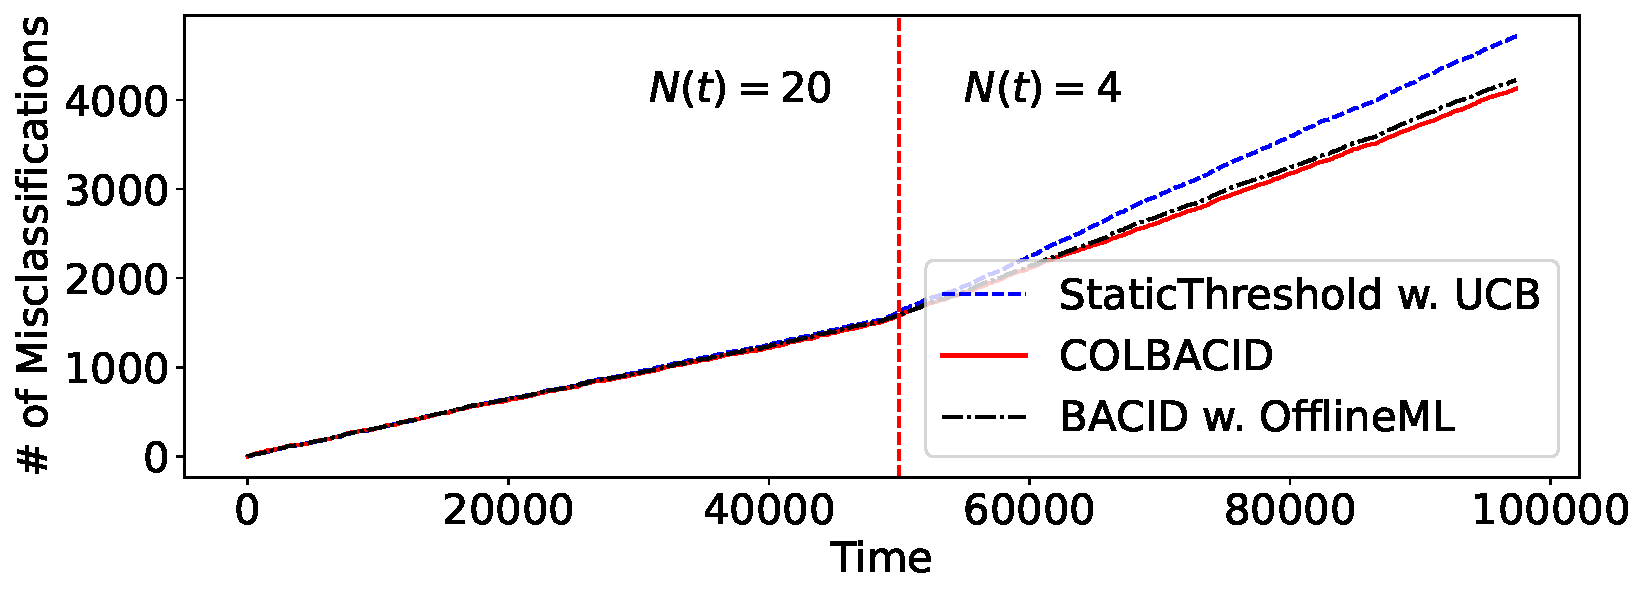
\includegraphics[width=4in]{figures/sim-horizon.pdf}
\caption{Number of misclassifications as a function of time with nonstationary reviewer capacity}
\label{fig:horizon}
\end{figure}

\begin{figure}[htbp]
  \centering
  \begin{minipage}{0.48\textwidth}
    \centering
    
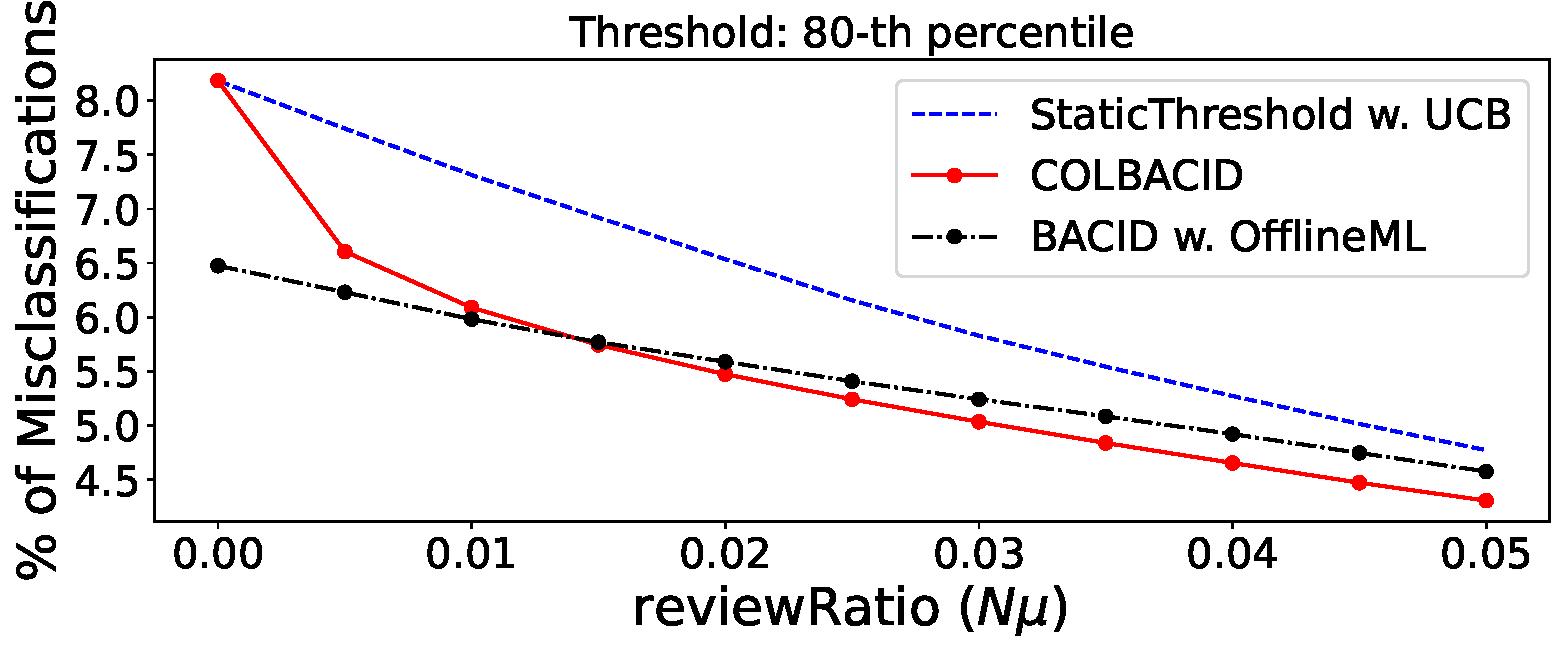
\includegraphics[width=3in]{figures/80.pdf}
  \end{minipage}%
  \\
  \begin{minipage}{1\textwidth}
    \centering
    \begin{tabular}{|l|c|c|c|c|c|}
    \hline
    \textbf{Review Ratio ($N\mu$)} & \textbf{0.01} & \textbf{0.02} & \textbf{0.03} & \textbf{0.04} & \textbf{0.05} \\
    \hline
    $\staticTh$  & 7.3\% & 6.5\% & 5.8\% & 5.3\% & 4.8\% \\
    \hline
    \textbf{$\conbacid$}                  & \textbf{6.1\%} & \textbf{5.5\%}  & \textbf{5.0\%} & \textbf{4.7\%} & \textbf{4.3\%} \\
    \hline
    BACID w.\ OfflineML       & 6.0\% & 5.6\% & 5.2\% & 4.9\% & 4.6\% \\
    \hline
  \end{tabular}
  \end{minipage}
\caption{Percentage of Misclassifications as a function of the review ratio}
\label{fig:80}
\end{figure}

\noindent
\textbf{Benefit of joint congestion awareness and online learning}. The second setting is a stationary setting with $N(t) \equiv N$ and we consider the percentage of misclassifications as a function of $N$ (or equivalently the review ratio $N\mu$) for the three algorithms. We vary $N \in \{0,1,\ldots,10\}$, so the range of considered review ratio is in $[0,5\%]$. Note that although Footnote~\ref{footnote:estimate} estimates a review ratio of $0.2\%$ to $1\%$ in Meta, we focus on a review ratio above $1\%$ because otherwise the number of content humans can review is at most $1000$ in our online dataset; at the scale of Meta this is not an issue as $0.2\%$ of a billion content pieces yields two millions of online samples per day.

Figure~\ref{fig:80} shows the percentage of misclassifications at the end of horizon for each algorithm. As discussed above, we fix the auto-deletion threshold to $80\%-$percentile maximum score in the offline dataset; Appendix~\ref{app:numerics} shows the results for other thresholds, which are similar to Figure~\ref{fig:80}. Consistently, $\conbacid$ outperforms $\staticTh$ by reducing more than $10\%$ misclassifications ($1 - 4.3\% / 4.8\%$ in the table of Figure~\ref{fig:80}). Moreover, when the review ratio is more than $1.5\%$, $\conbacid$ outperforms $\bacid$ w. OfflineML. This demonstrates the effectiveness of online learning when there is distribution shift between the offline dataset and the online dataset. Note that since $\conbacid$ only minimally uses the offline dataset for the auto-deletion threshold, it cannot have the same performance as $\bacid$ w. OfflineML when the online dataset is extremely small (review ratio less than $1\%$ in our simulation). As discussed above, this is not an issue for large social media platforms where millions of online samples are reviewed every day. Lastly, it is possible to further improve the numerical efficiency of $\conbacid$: in Appendix~\ref{app:numerics}, we simulate a variant of $\conbacid$ where instead of a FCFS scheduling, admitted content is scheduled based on the optimistically estimated loss $\bar{\ell}$. This algorithm shows better performance than $\conbacid$ when the review ratio is small.

\noindent \textbf{Importance of label-driven admission.} Motivated by our example in Section~\ref{sec:opti-fail}, the last setting shows that an optimism-only learning approach can fail to learn correct classification. Different from the above two settings, which set $\text{pView}_t \equiv 1$ for any content $t$, this setting varies this predicted number of views across content and studies how it impacts algorithms' performance. Specifically, for any non-policy-violating content $t \in \set{D}_{\text{online}}$, we set $\text{pView}_t \equiv P$ and vary $P \in \{1,\ldots,100\}.$ For policy-violating content $t$ we still set $\text{pView}_t \equiv 1.$ This setting captures practical scenarios where non-policy-violating content tends to have more views than policy-violating content. Fixing the review ratio to $0.05$, Figure~\ref{fig:misclass-selective} shows the percentage of misclassifications as a function of $P$ for both $\staticTh$, an optimism-only approach, and $\conbacid$, which contains a label-driven admission component. As Figure~\ref{fig:misclass-selective} shows, both $\staticTh$ and $\conbacid$ may increase their number of misclassifications as $P$ increases. However, $\conbacid$ is more robust and retains strong performance, while eventually $\staticTh$ fails to classify any policy-violating content (the percentage of policy-violating content in the online dataset is $8.2\%$). Figure~\ref{fig:nreview} explains why this happens. As $P$ increases, $\staticTh$ prioritizes more and more non-policy-violating content for reviews and thus eventually it will not review any policy-violating content. This mimics the phenomenon our theory predicts in Proposition~\ref{prop:fail-to-learn}. In contrast, thanks to the label-driven component, $\conbacid$ maintains a minimum number of human reviews for policy-violating content, although it has lower value ($\text{pView}_t$) to review.
\begin{figure}
\centering
%--- 1st panel ---------------------------------------------------
  \begin{subfigure}[b]{0.5\textwidth}
  \centering
    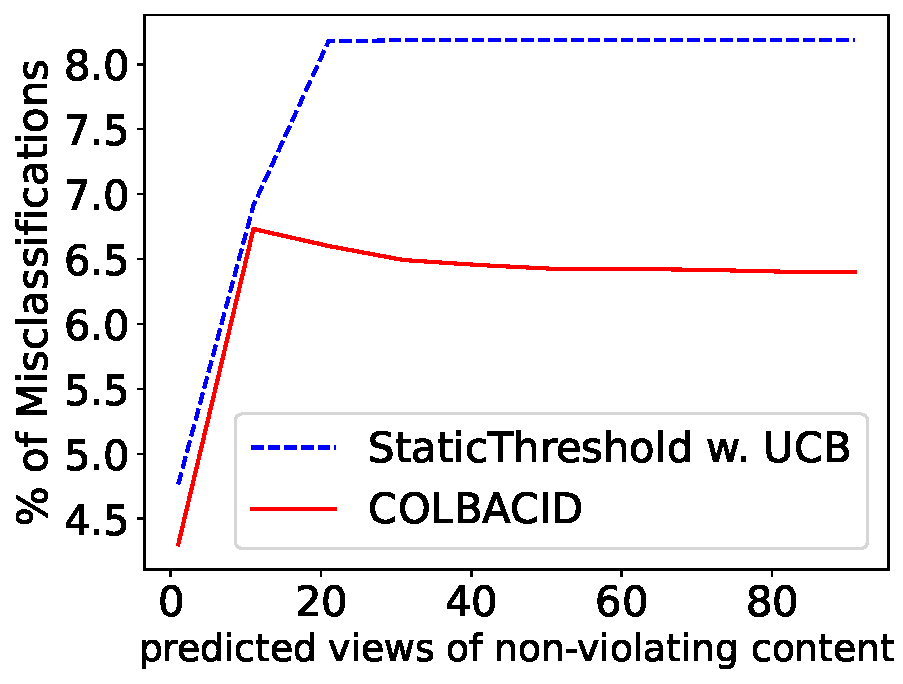
\includegraphics[width=2in]{figures/misclass-select.pdf}
    \caption{Percentage of misclassifications}
    \label{fig:misclass-selective}
  \end{subfigure}\hfill
  %--- 2nd panel ---------------------------------------------------
  \begin{subfigure}[b]{0.5\textwidth}
  \centering
    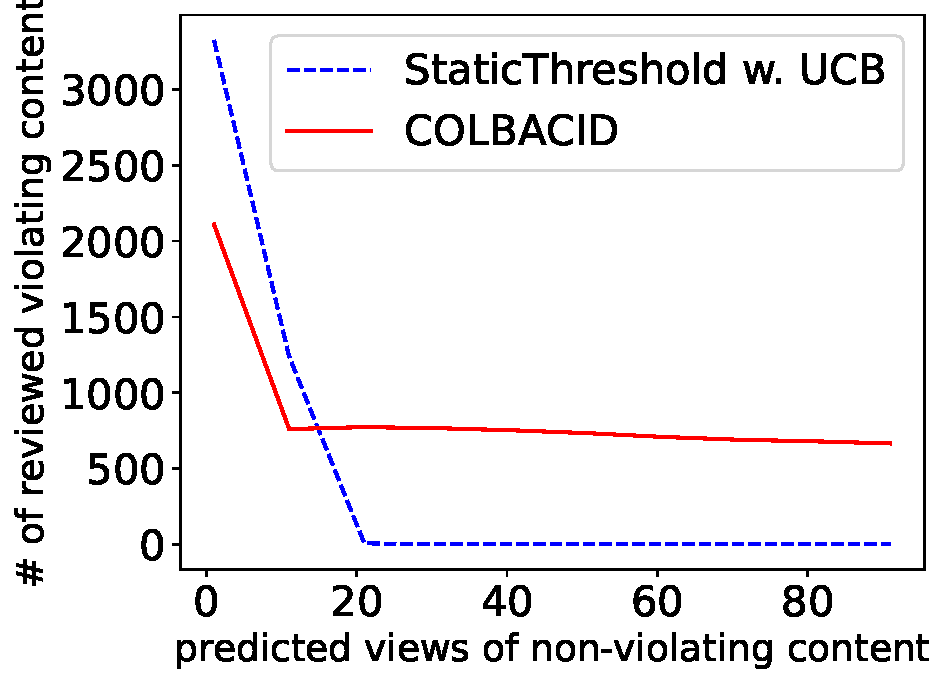
\includegraphics[width=2in]{figures/nreview-select.pdf}
    \caption{Number of reviewed violating content}
    \label{fig:nreview}
  \end{subfigure}
\caption{Algorithmic performance when non-violating content has more numbers of views}
\label{fig:selective}
\end{figure}